\documentclass{article}\usepackage{graphicx, color}
%% maxwidth is the original width if it is less than linewidth
%% otherwise use linewidth (to make sure the graphics do not exceed the margin)
\makeatletter
\def\maxwidth{ %
  \ifdim\Gin@nat@width>\linewidth
    \linewidth
  \else
    \Gin@nat@width
  \fi
}
\makeatother

\definecolor{fgcolor}{rgb}{0.2, 0.2, 0.2}
\newcommand{\hlnumber}[1]{\textcolor[rgb]{0,0,0}{#1}}%
\newcommand{\hlfunctioncall}[1]{\textcolor[rgb]{0.501960784313725,0,0.329411764705882}{\textbf{#1}}}%
\newcommand{\hlstring}[1]{\textcolor[rgb]{0.6,0.6,1}{#1}}%
\newcommand{\hlkeyword}[1]{\textcolor[rgb]{0,0,0}{\textbf{#1}}}%
\newcommand{\hlargument}[1]{\textcolor[rgb]{0.690196078431373,0.250980392156863,0.0196078431372549}{#1}}%
\newcommand{\hlcomment}[1]{\textcolor[rgb]{0.180392156862745,0.6,0.341176470588235}{#1}}%
\newcommand{\hlroxygencomment}[1]{\textcolor[rgb]{0.43921568627451,0.47843137254902,0.701960784313725}{#1}}%
\newcommand{\hlformalargs}[1]{\textcolor[rgb]{0.690196078431373,0.250980392156863,0.0196078431372549}{#1}}%
\newcommand{\hleqformalargs}[1]{\textcolor[rgb]{0.690196078431373,0.250980392156863,0.0196078431372549}{#1}}%
\newcommand{\hlassignement}[1]{\textcolor[rgb]{0,0,0}{\textbf{#1}}}%
\newcommand{\hlpackage}[1]{\textcolor[rgb]{0.588235294117647,0.709803921568627,0.145098039215686}{#1}}%
\newcommand{\hlslot}[1]{\textit{#1}}%
\newcommand{\hlsymbol}[1]{\textcolor[rgb]{0,0,0}{#1}}%
\newcommand{\hlprompt}[1]{\textcolor[rgb]{0.2,0.2,0.2}{#1}}%

\usepackage{framed}
\makeatletter
\newenvironment{kframe}{%
 \def\at@end@of@kframe{}%
 \ifinner\ifhmode%
  \def\at@end@of@kframe{\end{minipage}}%
  \begin{minipage}{\columnwidth}%
 \fi\fi%
 \def\FrameCommand##1{\hskip\@totalleftmargin \hskip-\fboxsep
 \colorbox{shadecolor}{##1}\hskip-\fboxsep
     % There is no \\@totalrightmargin, so:
     \hskip-\linewidth \hskip-\@totalleftmargin \hskip\columnwidth}%
 \MakeFramed {\advance\hsize-\width
   \@totalleftmargin\z@ \linewidth\hsize
   \@setminipage}}%
 {\par\unskip\endMakeFramed%
 \at@end@of@kframe}
\makeatother

\definecolor{shadecolor}{rgb}{.97, .97, .97}
\definecolor{messagecolor}{rgb}{0, 0, 0}
\definecolor{warningcolor}{rgb}{1, 0, 1}
\definecolor{errorcolor}{rgb}{1, 0, 0}
\newenvironment{knitrout}{}{} % an empty environment to be redefined in TeX

\usepackage{alltt}
\usepackage{graphicx, hyperref}
\usepackage[backend=bibtex, natbib=true]{biblatex}
\addbibresource{references/refs.bib}
\IfFileExists{upquote.sty}{\usepackage{upquote}}{}


\begin{document}

\part{Background}
\section{Networks}
\section{Visualization}
\section{Layout Algorithms}

\part{User Interface}
\section{Technical Aspects}
\subsection{Software}

Gravicom utilizes three main pieces of software to establish interactive user control of a random graph. The three pieces used are Shiny, D3, and igraph. They are used to manage server/client interaction, user interface and graph layout, and data formatting, respectively.

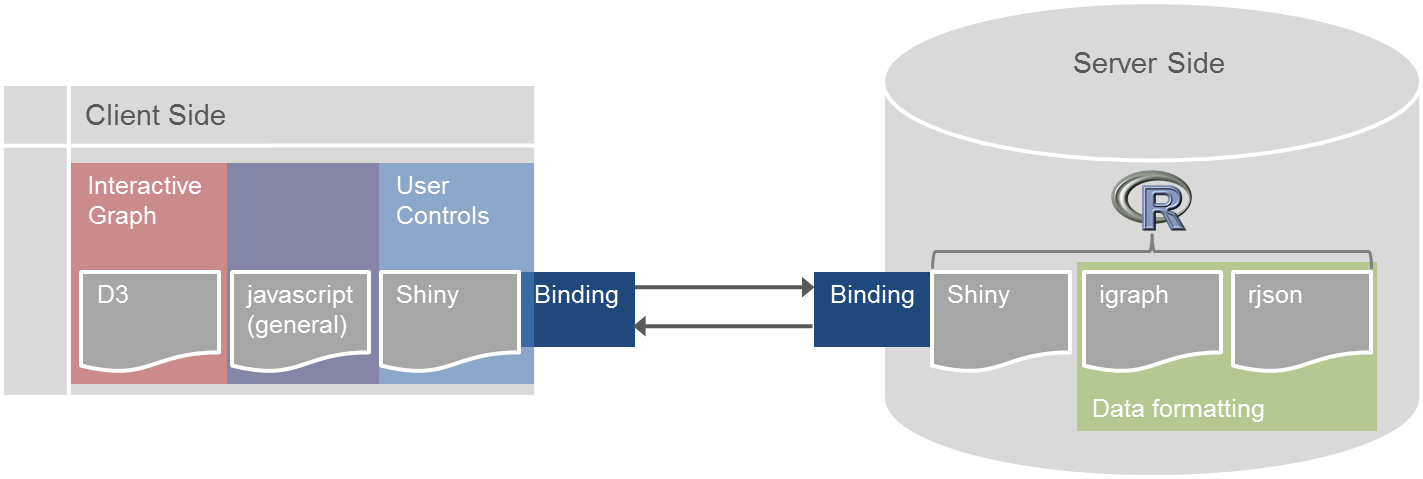
\includegraphics[width=.95\textwidth]{images/clientserverflow.png}


\subsubsection{Shiny}

Shiny is an R package created by RStudio that enables R users to create an interactive web application that utilizes R as the background engine.\cite{rs-shiny} Through default methods to build user interface elements in HTML and a handle to the server side code, Shiny is a very simple way to turn R code into a website. 

Gravicom uses the Shiny functionality to create user controls, pass correctly formatted data to the client, and as a means to display summary information regarding the user's interactions with a graph at any point in time. In this context, Shiny serves as the translator between the formatted data and what the user sees and interacts with on their screen.


\subsubsection{D3}

D3 is a javascript library written by Mike Bostock with the main purpose of visualizing and interacting with data and can be found at \url{http://www.d3js.org}.\cite{mb-d3} The title D3 stands for ``Data Driven Documents”. This library facilitates manipulation of HTML elements, SVG (scalable vector graphics), and CSS (cascading style sheets) with the end goal of animations and interactions that are tied to underlying data. The key idea behind the library is that DOM elements are completely determined by the data, so rather than adding elements to a web page to be viewed by users, D3 allows users to see and interact with graphical representaions of their data in a web framework. 

Gravicom uses D3 to handle all graphical displays and user interactions with the graph. The data is passed to the client and able to be used through Shiny's input bindings. It is crucial that the data has been formatted correctly at this point for the javascript to properly function. For this reason, we limit the file types being passed in to the tool to a robust graph-specific type.

At this point in the page lifecycle, the graph's nodes are tied to circles and the edges are tied to paths on the page. User manipulations such as selecting, dragging, and grouping are handled by D3 and then data is passed back to the server via Shiny's output bindings to allow for communication between user and the R engine underneath. What this means is that all visualization and user interaction with the graph are accomplished using javascript, more specifically the library D3. Shiny and R serve as the framework on which the data sits, but when the user touches the data they are doing so through the javascript pieces.


\subsubsection{igraph}

igraph is a software package used for creating and manipulating undirected and directed graphs.\cite{gc-igraph} It is a cross-language package available for C, R, python, and Ruby. igraph also supports multiple graph file formats and visualization of graph structures.

Gravicom utilizes two parts of igraph, first is the conversion from a gml file to an XML file. The gml file format, short for Graph Modelling Language, is a hierarchical ASCII-based file format for describing graphs. Here is an example gml file of an undirected graph with two nodes and one edge. The important points to note are the the node ids are numeric, the edge has only source and target attributes of the node ids to be connected, and the nodes can have other attributes, as typified by ``value" in the example.
\begin{knitrout}
\definecolor{shadecolor}{rgb}{0.969, 0.969, 0.969}\color{fgcolor}\begin{kframe}
\begin{verbatim}
## graph
## [
##   directed 0
##   node
##   [
##     id 0
##     label "Node 1"
##     value 100
##   ]
##   node
##   [
##     id 1
##     label "Node 2"
##     value 200
##   ]
##   edge
##   [
##     source 1
##     target 0
##   ]
## ]
\end{verbatim}
\end{kframe}
\end{knitrout}


Then, once we have an XML file we can convert to a JSON file using the R package rjson.\cite{acb-rjson} Getting the graphs in a JSON file formats makes working with them in the D3 library incredibly straightforward. Here is our example in the finalized JSON format.
\begin{knitrout}
\definecolor{shadecolor}{rgb}{0.969, 0.969, 0.969}\color{fgcolor}\begin{kframe}
\begin{verbatim}
## {
##   "nodes":
##   [{"id":"n0","v_id":"0","v_label":"Node 1","v_value":"100"}, 
##    {"id":"n1","v_id":"1","v_label":"Node 2","v_value":"200"}], 
##  "edges":
##   [{"source":0, "target":1}]
## }
\end{verbatim}
\end{kframe}
\end{knitrout}


igraph is also used to compute initial x and y coordinates for the graph using a force-driven layout prior to being passed to the force layout in D3. This reduces the initial work that must be done by the javascript library and helps minimize unnecessary movement by the nodes. This is critical as the extra movement at the loading of the pages creates an unnecessarily chaotic start to the user's experience.



\subsection{Data Management}
\section{Design and Functionality}

\part{Further Work}

\printbibliography
\end{document}
